\chapter{Bearing Design}

\section{Choose bearing type}
The reaction forces of bearings were calculated in Chapter 6. Since bearings selection is dependent on the ratio $ F_a/F_r $, the list below identifies the loads on each shaft:
\begin{itemize}
	\item On shaft 1, the radial loads are $ F_{1Bx} $, $ F_{1By} $, $ F_{1Dx} $, $ F_{1Dy} $; the axial load is $ F_{21z} $.
	\item On shaft 2, the radial loads are $ F_{2Ax} $, $ F_{2Ay} $, $ F_{2Dx} $, $ F_{2Dy} $; the axial load is $ F_{12z} + F_{31z} $.
	\item On shaft 3, the radial loads are $ F_{3Ax} $, $ F_{3Ay} $, $ F_{3Cx} $, $ F_{3Cy} $; the axial load is $ F_{22z} $.
\end{itemize}

Since shaft is simply supported beam (i.e. a shaft has pinned support at 1 end and roller support at the other end), the left side bearing carries both radial and axial forces while the right side bearing only carries radial force. \textbf{Table \ref{Fr/Fa}} summarizes the calculation of those loads (refer to \textbf{Table \ref{soltab}} for numerical values of the loads):

\begin{table}[ht]
	\centering
	\caption{Calculation table for limiting ratio $ F_a/F_r $}
	\begin{tabular}{lllllll}\toprule
		Sect. & $ F_x \unitp{kN} $ & $ F_y \unitp{kN} $ & $ F_z \unitp{kN} $ & $ F_r = \sqrt{F_x^2+F_y^2} \unitp{kN} $ & $ F_a = |F_z| \unitp{kN} $ & $ F_a/F_r $ \\ \midrule
		$ 1B $ & -5.88 & -0.1 & 0.22 & 5.88 & 0.22 & 0.04 \\
		$ 1D $ & 1.68 & -0.31 & 0 & 1.7 & 0 & - \\
		$ 2A $ & 1.14 & 0.08 & 0.47 & 1.14 & 0.47 & 0.42 \\
		$ 2D $ & 1.09 & -0.8 & 0 & 1.36 & 0 & - \\
		$ 3A $ & 1.76 & -0.22 & -0.69 & 1.77 & 0.69 & 0.39 \\
		$ 3C $ & -6.62 & 1.36 & 0 & 6.76 & 0 & -\\
		\bottomrule
	\end{tabular}
	\label{Fr/Fa}
\end{table}

The ratio $ F_a/F_r \geq 0.3 $ indicates the axial loads on shaft 2 and 3 are significant. Therefore, angular contact ball bearings, single row are selected for the 2 shafts. However, if the bearings are used, misalignment should not exist as recommended by the comparison table on p.72 \cite{rolling_bearings}. For shaft 1, it uses a pair of deep groove ball bearings.

The shafts are short in length, which is suitable for adjusted bearing arrangements since thermal expansion is small to axially displacing the bearings. \textbf{Figure \ref{bearing arrangement}} shows similar design and arrangement of the shafts in the speed reducer.

It is worth to mention that the actual radial load $ F_r $ and axial load $ F_a $ depend on both the bearing type and bearing arrangement. What computed in \textbf{Table \ref{Fr/Fa}} was the preliminary calculation to determine the suitable bearing type given the loads. The 'real' $ F_r $ and $ F_a $ shall be computed in the next section.

\begin{figure}[ht]
	\centering
	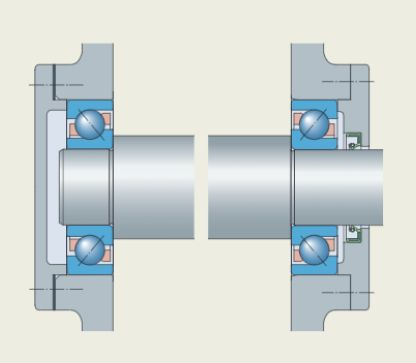
\includegraphics{bearing arrangement}
	\caption{Adjusted bearing arrangement, angular contact ball bearings arranged face-to-face. It requires proper adjustment of clearance or preload during mounting, p.76 \cite{rolling_bearings}}
	\label{bearing arrangement}
\end{figure}

Also from the previous chapter, the bore diameter $ d $ and available space $ b $ are also computed:
\[
\begin{array}{l}
d_{1B} = d_{1D} = 35 \unit{mm}, b_{O1} = 21 \unit{mm}\\
d_{2A} = d_{2D} = 45 \unit{mm}, b_{O2} = 21 \unit{mm}\\
d_{3A} = d_{3C} = 60 \unit{mm}, b_{O3} = 25 \unit{mm}\\
\end{array}
\]

From the specifications above, the bearings are selected from standard single row angular contact ball bearings product table, p.406 \cite{rolling_bearings}:
\begin{table}[ht]
	\centering
	\caption{Compact specification table of selected bearings according to SKF \cite{rolling_bearings}}
	\begin{tabular}{lll}\toprule
		Specifications & Bearings 2 & Bearings 3 \\ \midrule
		SKF designation & 7209 BE-2RZP & 7212 BEP\\
		$ d \unitp{mm} $ & 45 & 60\\
		$ D \unitp{mm} $ & 85 & 110\\
		$ B \unitp{mm} $ & 19 & 22\\
		$ C \unitp{kN} $ & 35.8 & 57.2\\
		$ C_0 \unitp{kN} $ & 26 & 45.5\\
		$ P_u \unitp{kN} $ & 1.12 & 1.93\\
		$ d_a \unitp{mm} $ min. & 52 & 60\\
		$ d_a \unitp{mm} $ max. & 65 & -\\
		$ D_a \unitp{mm} $ max. & 78 & 101\\
		$ r_a \unitp{mm} $ max. & 1 & 1.5\\
		$ k_r $ & 0.095 & 0.095\\
		\bottomrule
	\end{tabular}
	\label{bearingspecs}
\end{table}

\begin{figure}[ht]
	\centering
	\begin{subfigure}{.4\linewidth}
		\centering
		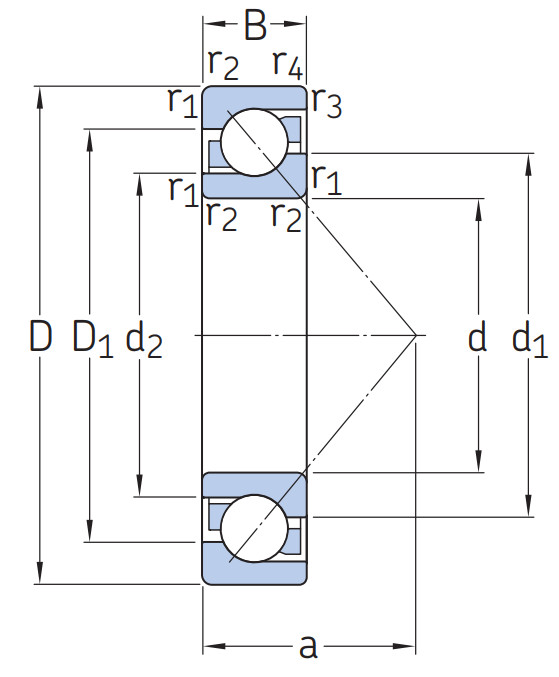
\includegraphics[width=\linewidth,keepaspectratio=true]{bearing dimension}
		\caption{Front view of single row angular contact ball bearings}
		\label{bearingdim}
	\end{subfigure}\hspace*{0.1\linewidth}
	\begin{subfigure}{.4\linewidth}
		\centering
		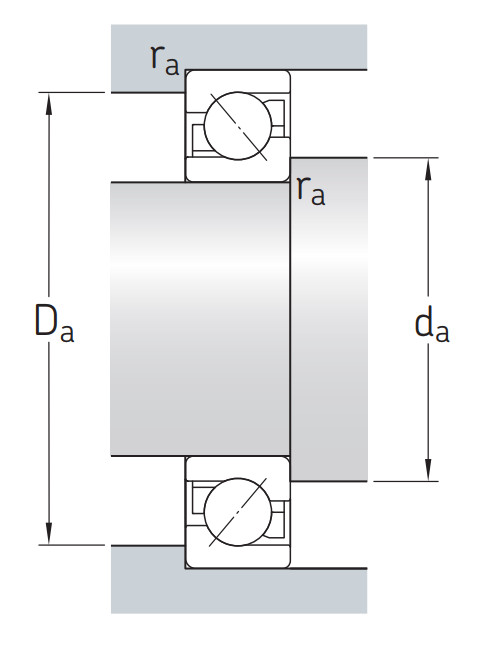
\includegraphics[width=\linewidth,keepaspectratio=true]{bearing assembly}
		\caption{Important dimensions in assembly of shaft and single row angular contact ball bearings in a housing unit}
		\label{bearingass}
	\end{subfigure}
	\caption{Important dimensions in assembly of single row angular contact ball bearings \cite{rolling_bearings}}
	\label{bearingdimass}
\end{figure}

where
\begin{itemize}
	\item $ D, B, d_a, D_a, r_a $ are the dimensions, specified in \textbf{Figure \ref{bearingdimass}}.
	\item $ C $ is the basic dynamic load rating,$ \unit{kN} $.
	\item $ C_0 $ is the basic static load rating,$ \unit{kN} $.
	\item $ P_u $ is the fatigue load limit,$ \unit{kN} $.
	\item $ k_r $ is the calculation factor.
\end{itemize}

Referring to \textbf{Table \ref{safety-sigma}} and \textbf{\ref{safety-tau}}, the fillet radius and shoulder diameter are in accordance with the limits provided in \textbf{Table \ref{bearingspecs}}.

\section{SKF rating life for shaft 2, 3}
SKF uses a modified life factor in accordance with ISO 281 to optimize prediction of bearing life, p.89 \cite{rolling_bearings}. In terms of operating hours, the SKF rating life $ L_{nmh} $ (unit is$ \unit{h} $) is
\[L_{nmh} = \left(\dfrac{10^6}{60n}\right) a_1 a_{SKF} \left(\dfrac{C}{P}\right)^p\]
where
\begin{itemize}
	\item $ n $ is the speed of the shaft on which the bearing is mounted,$ \unit{rpm} $. The value is provided in \textbf{Table \ref{tab:my-table}}.
	\item $ a_1 $ is the life adjustment factor for reliability, Table 3, p.90 \cite{rolling_bearings}. The bearings are evaluated at $ 90\% $ reliability for common machinery. Therefore, $ a_1 = 1 $.
	\item $ a_{SKF} $ is the life modification factor, $ a_{SKF} $. The value relies on many other factors, as shown in Diagram 9, p.96 \cite{rolling_bearings}.
	
	In the diagram, the horizontal value is $ \eta_c \dfrac{P_u}{P} $, where $ \eta_c $ is the contamination factor, provided in Table 6, p.105 \cite{rolling_bearings} ($ \eta_c = 0.5 $ for normal cleanliness, chosen at worst case); $ P_u $ is the fatigue load limit, which was given in \textbf{Table \ref{bearingspecs}}; $ P $ is the equivalent dynamic bearing load, which shall be mentioned below. 
	
	The curves in the diagram correspond to a value of $ \kappa $, where $ \kappa $ is the lubrication condition (viscosity ratio) of the bearing. The value $ \kappa $ is calculated using equation on p.102 \cite{rolling_bearings}:
	\[
	\kappa = \dfrac{\nu}{\nu_1}
	\]
	where
	\begin{itemize}
		\item $ \nu $ is the actual operating viscosity of the oil or grease based oil,$ \unit{mm^2/s} $. The value depends on operating temperature, as given in Diagram 13, p.100 \cite{rolling_bearings}. Industrial machines usually operate at $ 40\degc $, however the viscosity will be considered at $ 80\degc $ in worst case. The mineral oil is ISO VG 46, which is a high quality industrial oil commonly used for mechanical lubrication. Therefore, the viscosity is $ \nu = 30 \unit{mm^2/s} $.
		\item $ \nu_1 $ is the rated viscosity, function of the mean bearing diameter and rotational speed,$ \unit{mm^2/s} $. The value is evaluated as shown in Diagram 14, p.101 \cite{rolling_bearings}. The variable in the horizontal axis is bearing mean diameter $ d_m, \unit{mm} $. It is calculated using bore diameter $ d $ and outer diameter $ D $, p.102 \cite{rolling_bearings} (all of which have been mentioned above). On the page, additional considerations are also mentioned. If the factor $ nd_m\leq 10000\unit{mm/min} $, EP (extreme pressure) and AW (anti-wear) additives are needed to reduce wear. If $ nd_m \geq 500,000\unit{mm/min} $ for $ d_m < 200 \unit{mm} $ or $ nd_m \geq 400,000 \unit{mm/min} $ for $ d_m > 200 \unit{mm} $, operating temperature must be given more attention. Since the factors in 3 shafts are outside these conditions, it is therefore omitted.
		\begin{table}[ht]
			\centering
			\caption{Calculation table for lubrication condition $ \kappa $}
			\begin{tabular}{llllllll}\toprule
				Shaft & $ d $ & $ D $ & $ d_m = 0.5(d+D) $ & $ n \unitp{rpm} $ & $ nd_m \unitp{mm/min} $ & $ \nu_1 \unitp{mm^2/s} $ & $ \kappa $ \\\midrule
				2 & 45 & 85 & 65 & 514.42 & 33437.31 & 30 & 1.17\\
				3 & 60 & 110 & 90 & 181.88 & 16368.75 & 48 & 0.73\\\bottomrule
			\end{tabular}
		\end{table}
	\end{itemize}
	
	To summarize the results, \textbf{Table \ref{askf}} is provided below:
	\begin{table}[ht]
		\centering
		\caption{Calculation table life modification factor $ a_{SKF} $}
		\begin{tabular}{llllll}\toprule
			Sect. & $ P_u \unitp{kN} $ & $ P \unitp{kN} $ & $ \eta_c \dfrac{P_u}{P} $ & $ \kappa $ & $ a_{SKF} $ \\ \midrule
			$ 2A $ & 1.12 & 1.78 & 0.32 & 0.43 & 1.1\\
			$ 2D $ & 1.12 & 2.28 & 0.25 & 0.43 & 0.9\\
			$ 3A $ & 1.93 & 2.76 & 0.35 & 0.27 & 0.22\\
			$ 3C $ & 1.93 & 7.6  & 0.13 & 0.27 & 0.2\\
			\bottomrule
		\end{tabular}
		\label{askf}
	\end{table}
	\item $ C $ is the basic dynamic load rating,$ \unit{kN} $. The value is provided in \textbf{Table \ref{bearingspecs}}.
	\item $ P $ is the equivalent dynamic bearing load,$ \unit{kN} $. It is calculated using the formula on p.398 \cite{rolling_bearings} multiplied by the gear factor 1.05 (pitch and form errors $ < 0.02 \unit{mm} $, p.93 \cite{rolling_bearings}). For the necessary factors $ X,Y,e $, Table 10 on p.400 \cite{rolling_bearings} is used for bearings pairs arranged face-to-face:
	\begin{figure}[ht]
		\centering
		\begin{subfigure}{.4\linewidth}
			\centering
			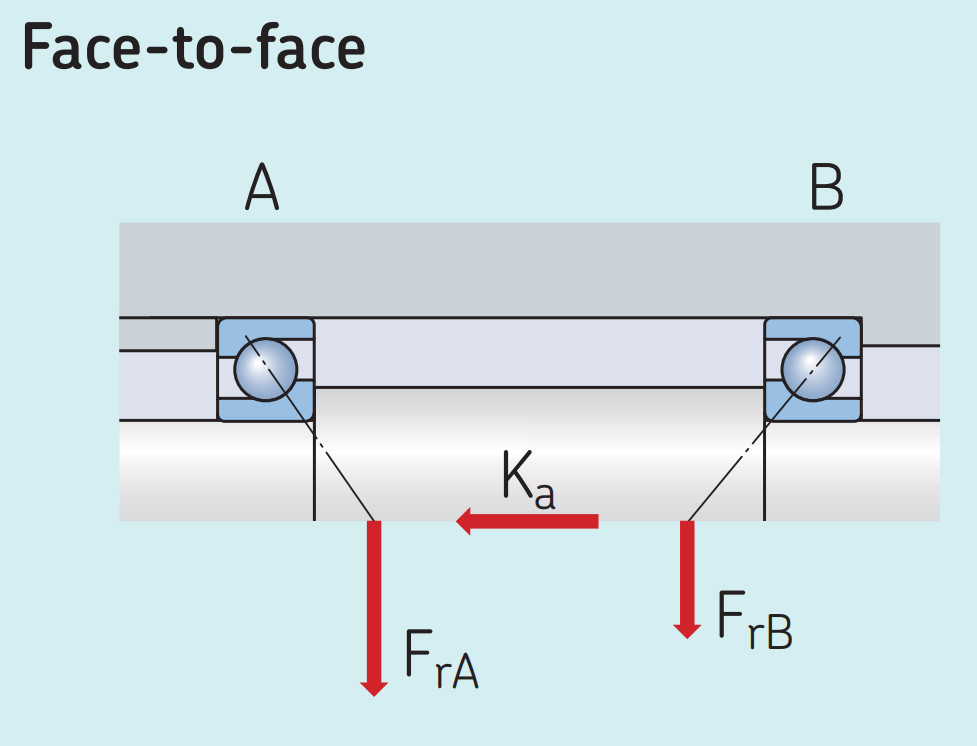
\includegraphics[width=\linewidth,keepaspectratio=true]{face2face}
			\caption{$ K_a $ points to the left}
			\label{face2face}
		\end{subfigure}\hspace*{0.1\linewidth}
		\begin{subfigure}{.4\linewidth}
			\centering
			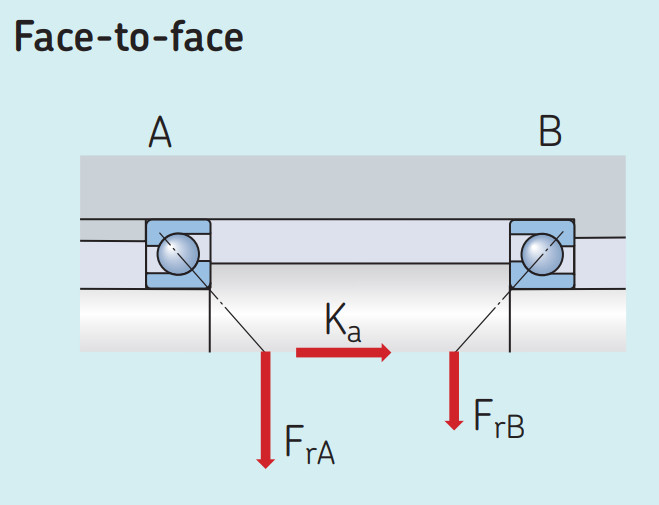
\includegraphics[width=\linewidth,keepaspectratio=true]{face2face2}
			\caption{$ K_a $ points to the right}
			\label{face2face2}
		\end{subfigure}
		\caption{Face-to-face force distribution of single row angular contact ball bearings \cite{rolling_bearings}}
	\end{figure}
	\[
	\left\{
	\begin{array}{l}
	P = 1.05(F_r + 0.55F_a), F_a/F_r \leq 1.14\\
	P = 1.05(0.57F_r + 0.93F_a), F_a/F_r > 1.14
	\end{array}
	\right.
	\]
	where
	\begin{itemize}
		\item $ F_a $ is the axial force,$ \unit{N} $. The value is computed according to Table 11, p.401 \cite{rolling_bearings}. All 3 bearings are B-series as designated on p.404 \cite{rolling_bearings}, therefore they have $ 40^\circ $ contact angle. This value corresponds to factor $ R = 0.88 $. Following the provided conditions and the direction of $ F_z $ (all units are in$ \unit{kN} $), \textbf{Table \ref{bearingforce}} is obtained:
		\begin{table}[ht]
			\centering
			\caption{Compact specification table of selected bearings according to SKF \cite{rolling_bearings}}
			\begin{tabular}{lllllll}\toprule
				Shaft & $ F_{rA} $ & $ F_{rB} $ & $ K_a = |F_z| $ & $ R(F_{rB}-F_{rA}) $ & $ F_{aA} $ & $ F_{aB} $ \\\midrule
				1 & 1.14 & 1.09 & 0.47 (\textbf{Fig. \ref{face2face}})& 0.19 (case 1b) & 1 & 1.48 \\
				2 & 1.76 & 6.62 & 0.69 (\textbf{Fig. \ref{face2face2}})& 4.38 (case 2c) & 1.56 & 0.87 \\\bottomrule
			\end{tabular}
			\label{bearingforce}
		\end{table}
	
		where $ F_{rA} $ and $ F_{rB} $ are the radial forces of the left and right bearings, respectively.
		\item $ F_r $ is the radial force,$ \unit{kN} $. The value is provided in \textbf{Table \ref{bearingspecs}}. It is required that $ F_r $ must be larger than the minimum radial load $ F_{rm} $, which is calculated as
		\[
		F_{rm} = k_r \left(\dfrac{\nu n}{1000}\right)^{2/3}(\dfrac{d_m}{100})^2
		\]
		where
		\begin{itemize}
			\item $ k_r $ is a calculation factor, which is given in \textbf{Table \ref{bearingspecs}}.
			\item $ \nu $ is the actual operating viscosity of the oil, which was mentioned above.
			\item $ n $ is the shaft speed, which was mentioned above.
			\item $ d_m $ is the bearing mean diameter,$ \unit{mm} $. The value is computed in Table
			\begin{table}[ht]
				\centering
				\caption{Condition check for radial load for bearing pairs arranged face-to-face}
				\begin{tabular}{lllllllll}\toprule
					Shaft & $ k_r $ & $ d $ & $ D $ & $ d_m = 0.5(d+D) $ & $ F_{rA} $ & $ F_{rB} $ & $ F_{rm} $ & Condition $ F_r \geq F_{rm} $ \\\midrule
					2 & 0.095 & 45 & 85 & 65 & 1.14 & 1.09 & 0.14 & Satisfied \\
					3 & 0.095 & 60 & 110 & 90 & 1.76 & 6.62 & 0.14 & Satisfied \\\bottomrule
				\end{tabular}
				\label{Frm}
			\end{table}
		\end{itemize}
	\end{itemize}
	In total, the equivalent dynamic bearing load on each bearing is shown in \textbf{Table \ref{Pload}} (the units are in$ \unit{kN} $ except for ratio $ F_a/F_r $, which is dimensionless):
	\begin{table}[ht]
		\centering
		\caption{Calculation table for equivalent dynamic bearing load $ P $}
		\begin{tabular}{lllll}\toprule
			Sect. & $ F_r $ & $ F_a $ & $ F_a/F_r < e $ & $ P \unitp{kN} $ \\ \midrule
			$ 2A $ & 1.14 & 1 & 0.88<1.14 & 1.78 \\
			$ 2D $ & 1.36 & 1.48  & 1.09<1.14 & 2.28 \\
			$ 3A $ & 1.77 & 1.56 & 0.88<1.14 & 2.76 \\
			$ 3C $ & 6.76 & 0.87 & 0.13<1.14 & 7.6 \\
			\bottomrule
		\end{tabular}
		\label{Pload}
	\end{table}
	\item $ p $ is the exponent of the life equation. For ball bearings, $ p = 3 $.
\end{itemize}

\begin{table}[ht]
	\centering
	\caption{Calculation table for SKF rating life $ L_{nmh} $ in hours}
	\begin{tabular}{llllll}\toprule
		Sect. & $ n \unitp{rpm} $ & $ a_{SKF} $ & $ C \unitp{kN} $ & $ P \unitp{kN} $ & $ L_{nmh} \unitp{h} $ \\ \midrule
		$ 2A $ & 514.42 & 1.1  & 35.8 & 1.78 & $ 291071.18 $ \\
		$ 2D $ & 514.42 & 0.9  & 35.8 & 2.28 & $ 113384.06 $ \\
		$ 3A $ & 181.88 & 0.22 & 66.3 & 2.76 & $ 277974.62 $ \\
		$ 3C $ & 181.88 & 0.2  & 66.3 & 7.6 & $ 12184.16 $ \\
		\bottomrule
	\end{tabular}
	\label{ratinglife}
\end{table}

\section{SKF rating life for shaft 1}
For shaft 1, the calculation is almost the same as the above.

\begin{table}[ht]
	\centering
	\caption{Compact specification table of shaft 1 bearings according to SKF \cite{rolling_bearings}}
	\begin{tabular}{ll}\toprule
		Specifications & Bearings 1 \\\midrule
		SKF designation & 6207 \\
		$ d \unitp{mm} $ & 35\\
		$ D \unitp{mm} $ & 72\\
		$ B \unitp{mm} $ & 17\\
		$ C \unitp{kN} $ & 27\\
		$ C_0 \unitp{kN} $ & 15.3\\
		$ P_u \unitp{kN} $ & 0.655\\
		$ d_a \unitp{mm} $ min. & 42 \\
		$ d_a \unitp{mm} $ max. & - \\
		$ D_a \unitp{mm} $ max. & 65 \\
		$ r_a \unitp{mm} $ max. & 1 \\
		$ k_r $ & 0.025\\
		$ f_0 $ & 14\\
		\bottomrule
	\end{tabular}
	\label{bearingspecs2}
\end{table}

Before evaluating SKF rating life, the axial load on the deep groove bearings must met this condition, p.254 \cite{rolling_bearings}:
\[
F_a = 0.22 \leq 0.25C_0 = 0.25\times  =3.83 \unitp{kN}
\]

Minimum load condition must also be evaluated, p.254 \cite{rolling_bearings}:
\[
\begin{array}{ll}
F_{rm} & = k_r\left(\dfrac{\nu n}{1000}\right)^{2/3}\left(d_m/100\right)^2\\
& = 0.025\times \left (\dfrac{30 \times 1455}{1000}\right)^{2/3} \left[\dfrac{0.5(35+72)}{100}\right]^2\\
& = 0.09<5.88\unitp{kN}
\end{array}
\]

where $ \nu $ and formula of $ d_m $ are taken from the previous section.

The bearing pair is arranged face-to-face. Therefore, using equation on p.254 \cite{rolling_bearings}:
\[
\begin{array}{l}
F_a/F_r = 0.1/5.88 = 0.017 \leq e = 0.27\\
\Rightarrow P = F_r + Y_1F_a = 5.88+2.45\times 0.1 = 6.13 \unitp{kN}
\end{array}
\]

where $ e, Y_1 $ are the calculation factors. They are provided on Table 10, p.257 \cite{rolling_bearings}, which relies on $ f_0,F_a,C_0 $.

The SKF rating life $ a_{SKF} $ is found using the same method applied to shaft 2 and 3 bearing pairs. First, the viscosity ratio $ \kappa $ is calculated:
\[
\kappa = \dfrac{\nu}{\nu_1} = \dfrac{30}{0.1} = 300
\]

Taking the same contamination factor $ \eta_c = 0.5 $, the ratio $ \eta_c \frac{P_u}{P} = 0.5\times \dfrac{0.655}{6.13} = 0.05 $.

From the value $ \kappa $ and $ \eta_c \frac{P_u}{P} $, $ a_{SKF} = 50 $. Using this value,
\[
\begin{array}{ll}
L_{nmh} & = \left(\dfrac{10^6}{60n}\right) a_1 a_{SKF} \left(\dfrac{C}{P}\right)^p\\
& = \left(\dfrac{10^6}{60\times}\right) \times 1 \times 50 \left(\dfrac{27}{6.13}\right)^3\\
& = 48940.2 \unitp{h}
\end{array}
\]

According to calculation, under specified environmental conditions (normal cleanliness, working at $ 80\degc $ and $ 90\% $ reliability), the bearings are guaranteed to operate for at least $ 12,000 $ hours. This is the typical life span in machines for use 8 hours a day, but not always fully utilized, Table 1, p.88 \cite{rolling_bearings}.

SKF recommends when $ \kappa < 1 $, EP/AW additives should be used, p.102 \cite{rolling_bearings}. However, it is always possible to obtain higher lubrication condition $ \kappa $ if better viscosity oil is used (ISO VG 63). Also, the speeds of 3 shafts are not too low ($ > 10 \unitp{rpm} $) that static loading analysis is needed. Therefore, the selected SKF bearings are still valid.

The proposed bearings are listed as follows (specifications are provided in SKF bearings catalog \cite{rolling_bearings}):
\begin{itemize}
	\item Shaft 1: 6207
	\item Shaft 2: 7209 BE-2RZP
	\item Shaft 3: 7212 BEP
\end{itemize}